\chapter{实例抽取}
对于一项活动,除了

\section{活动类别抽取}
\subsection{简单规则匹配}
\subsection{引入句法分析}
对错误结果的分析发现,大约有12\%的错误分类是因为活动表述的语法结构比较复杂,简单的规则匹配无法正确识别句子的主干。一种情况是,活动以主谓结构出现,如``麻辣烫真是太好吃了'',应该提取出``吃麻辣烫'';还有一种情况是动宾结构比较复杂,无法匹配比如``陪父母看了一场周星驰拍的很有意思的电影'',应该抽取出``陪父母''和``看电影''。为了正确处理这些情况,我们需要对句子进行句法分析,组织成依存树。

Stanford Parser(http://nlp.stanford.edu/software/lex-parser.shtml)是斯坦福大学自然语言处理组开发的句法分析工具。它主要提供英语语言的解析,但是也提供中文、德语、阿拉伯语等多语种的解析,但它的处理结果并不非常直观。最终本文选择哈尔滨工业大学开源的语言技术平台(Language Technology Platform, LTP)\cite{che2010ltp}作为句法分析工具。LTP提供分词、词性标注、命名实体识别、依存句法分析、语义角色标注等功能,提供自然语言处理的集成解决方案。

\begin{figure}[!h]
\centering
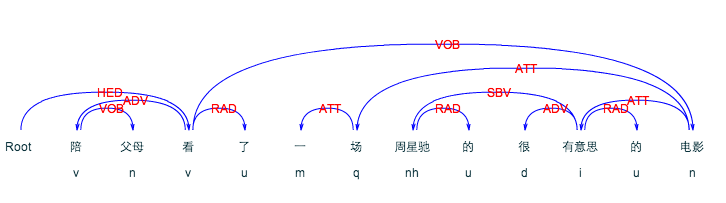
\includegraphics[width=0.9\textwidth]{ltpdemo1.png}
\caption{LTP句法分析结果}
\label{fig:ltp_demo}
\end{figure}


\subsection{局限}

\section{地点抽取}

我们与搜狐合作,得到的国内主要城市的兴趣点(POI, point of interest)数据,来辅助我们的地点抽取。

\section{情感极性分析}
如果抽取后发现微博中包含用户参与的一项活动,我们希望了解用户参与这项活动时的心情状态如何,帮助我们发现活动本身是正面还是负面,因此,需要对微博进行情感分析。

\subsection{方法概述}
观念挖掘和情感分析是信息检索中的一个重要领域,由于我们需要判断情感极性,因此是文档级的情感分类问题(Document-level sentiment classification)。

在本文的研究中,情感分类并不是一个主要工作,因此我们采用了比较简单的方法。从知网(HowNet, http://www.keenage.com/)提供了中文情感词典,其中包含

\subsection{实验结果与分析}
我们标注了20829条包含活动信息的微博,根据其情感极性标注为5级,-2为很负面,-1为一般负面,0为中性,1为一般积极,2为很积极。
按照

这种方法

\chapter{活动关系抽取及知识发现}
\section{xxx}
